\documentclass[conference]{IEEEtran}
\IEEEoverridecommandlockouts
\usepackage{cite}
\usepackage{amsmath}
\usepackage{graphicx}
\usepackage{booktabs}
\usepackage{multirow}
\usepackage{xcolor}
\usepackage{url}
\usepackage{textcomp}
\def\BibTeX{{\rm B\kern-.05em{\sc i\kern-.025em b}\kern-.08em
    T\kern-.1667em\lower.7ex\hbox{E}\kern-.125em X}}

\begin{document}

\title{Mining Human--AI Collaboration in Software Engineering Repositories: Outcomes and Collaboration Patterns of AI-Agent Pull Requests}

\author{\IEEEauthorblockN{Saman Shaheen}
\IEEEauthorblockA{\textit{Polytechnique Montr\'eal}\\
Montr\'eal, Canada\\
saman.shaheen@etud.polymtl.ca}
\and
\IEEEauthorblockN{[\'Emilie Larocque]}
\IEEEauthorblockA{\textit{Polytechnique Montr\'eal}\\
Montr\'eal, Canada\\
\relax[emilie.larocque@etud.polymtl.ca]}
\and
\IEEEauthorblockN{[Eugenia Carcea]}
\IEEEauthorblockA{\textit{Polytechnique Montr\'eal}\\
Montr\'eal, Canada\\
\relax[eugenia.carcea@etud.polymtl.ca]}
\and
\IEEEauthorblockN{[Randy M\'egane Rakotondrazafy]}
\IEEEauthorblockA{\textit{Polytechnique Montr\'eal}\\
Montr\'eal, Canada\\
\relax[randy-megane.rakotondrazafy@etud.polymtl.ca]}
}

\maketitle

\begin{abstract}
AI coding agents now open pull requests (PRs) on GitHub on their own, yet little is known about how maintainers treat them compared with human contributors. We study two questions: how \emph{development outcomes} (RQ1) and \emph{collaboration patterns} (RQ2) differ between AI-agent and human PRs. We mine 21{,}740 PRs (16{,}287 AI, 5{,}453 human) from the AIDev dataset, enrich them with comments and reviews through the GitHub GraphQL API, remove bot noise, and compare the groups with chi-square and Mann--Whitney U tests plus effect sizes. AI PRs are merged less often (72.9\% vs.\ 80.8\%; odds ratio 0.64) but, when merged, far faster (median 2.7 minutes vs.\ 4.6 hours). They also attract much less human interaction: the median AI PR has no comments or reviews, and only 13.5\% receive an approving review versus 47.5\% of human PRs. These patterns suggest that AI PRs are often handled as delegated output rather than discussed like teammates' contributions. Limitations in bot filtering and timestamp handling temper two of our metrics.
\end{abstract}

\begin{IEEEkeywords}
AI teammates, pull requests, mining software repositories, human--AI collaboration, code review
\end{IEEEkeywords}

\section{Introduction}
Autonomous coding agents such as OpenAI Codex, Devin, GitHub Copilot, Cursor and Claude Code no longer only suggest code: they open pull requests (PRs) that humans must review, discuss and merge~\cite{li2025rise}. Whether such agents behave like \emph{teammates} depends on what happens after the PR is opened. Is it accepted, how quickly, and how much interaction does it trigger? Repositories record exactly this trace (merge status, timestamps, reviews, comments), which makes mining software repositories (MSR) a natural way to study human--AI collaboration at scale. This report compares AI-agent and human PRs along two of the five suggested dimensions: development outcomes and collaboration patterns.

\section{Research Questions}
\textbf{RQ1 (Development outcomes).} How do AI-agent PRs differ from human PRs in merge rate, closing rate, time to merge, and number of reviews?

\textbf{RQ2 (Collaboration patterns).} How do developers communicate and what are the development communication skills?

The AI-agent PRs and human PRs were compared in terms of
A comment is a message that is typically sent to the poster immediately upon seeing a post.A comment is a message that is generally sent to the poster at the time of the post.
time, back and forth and clarification/approval/rejection language?

\noindent (RQ numbering follows the assignment handout.)

\section{Methodology}
\subsection{Data collection}
We use the AIDev dataset released with~\cite{li2025rise} (Hugging Face \texttt{hao-li/AIDev}, revision v3), the dataset behind the course repository \texttt{SAILResearch/AI\_Teammates\_in\_SE3}. It lists PRs opened by AI coding agents and, as a baseline, human PRs. We concatenated both tables, removed duplicate PR ids, kept all human PRs, and drew a random 50\% sample of the (much larger) AI table (seed 42). Each PR URL was parsed into owner/repository/number, and every PR was queried through the GitHub GraphQL API~\cite{githubgql} (15 PRs per request) for state, creation/close/merge timestamps, author login and account type, issue comments (first 100), reviews (first 50: state, submission time, body, author) and inline review comments (first 50 per review). The script waits for the rate-limit reset and retries failed batches. Of 23{,}416 sampled PRs, 22{,}710 were retrieved; 706 (3.0\%) no longer resolve (deleted or renamed repositories, disabled PRs) and were dropped. Mining ran in late September 2026.

\emph{Replication package:} \url{https://github.com/Eugenia3/Replication_Project_LOG6307E} (Colab pipeline, data archive, and this report).

\subsection{Cleaning and classification}
\textbf{AI vs.\ human.} We rely on AIDev's group label (PR opened by one of the dataset's AI agents vs.\ a human-authored PR) rather than our own heuristic. \\
\textbf{Bots.} Comments and reviews written by bots (login ending in \texttt{[bot]}, GraphQL type \texttt{Bot}, deleted accounts, or a list of common CI/dependency-bot names) are removed from every PR. Bot-authored \emph{PRs} are discarded only from the human group (970 PRs, 15.1\% of 6{,}423), because agents themselves often post from bot-flagged accounts and discarding them would empty the AI group. The final dataset contains 21{,}740 PRs (including 16{,}287 AI, 5{,}453 human). \\
\textbf{Missing values.} PRs without any timestamped comment have no response time (excluded from that test only); time to merge exists only for merged PRs; counts default to 0. \\
\textbf{Text.} Before counting words and matching keywords, comment bodies are stripped of HTML comments, code blocks, inline code, images, quoted lines, HTML tags and URLs. \\
\textbf{Language classes.} Three hand-written regular-expression lexicons flag explanation requests (e.g., ``is this intentional'', ``could you elaborate and explain''), approval (``LGTM'', ``looks good'', ``approved'') and rejection (``please fix/revert'', ``do not merge'', ``incorrect'') in any comment or review. Task-type classification was not needed for RQ1/RQ2.

\subsection{Metrics}
Table~\ref{tab:metrics} defines the per-PR metrics; all are computed after cleaning.

\begin{table}[t]
\caption{Metric definitions (one value per PR).}
\label{tab:metrics}
\centering\small
\begin{tabular}{@{}p{0.95in}p{2.4in}@{}}
\toprule
Metric & Definition \\
\midrule
Merge / close rate & Share of PRs with a merge / close timestamp (closed includes merged) \\
Time to merge & mergedAt $-$ createdAt, hours (merged PRs only) \\
Reviews & Number of non-bot reviews \\
Comments & Issue comments + reviews + inline review comments (non-bot) \\
Reviewers / participants & Distinct review authors / distinct authors of any comment or review \\
Comment length & Mean words per non-empty cleaned comment \\
First response$^\dagger$ & Earliest timestamped comment $-$ createdAt, hours \\
Alternations$^\dagger$ & Switches between PR author and others in the chronological comment sequence \\
Language flags & $\geq$1 clarification / approval / rejection match in the PR \\
Review outcome & $\geq$1 review in state APPROVED / CHANGE\_REQUESTED\\
\bottomrule
\end{tabular}
\\[2pt]\footnotesize $^\dagger$ See Threats to Validity:  The data lacks time stamps and is affected by bot-filtering issues. 
\end{table}

\subsection{Analysis}
Binary metrics are compared with $\chi^2$ tests of independence (SciPy default, Yates correction for $2{\times}2$ tables) and numeric metrics with two-sided Mann--Whitney U tests~\cite{mannwhitney}, because the distributions are skewed and zero-inflated. With $N\approx 21{,}700$ almost any difference is significant, so we also report effect sizes computed from the test outputs: the odds ratio (OR) for binary metrics and the probability of superiority $P(\mathrm{AI}{>}\mathrm{H})=U/(n_{AI}n_{H})$ for numeric ones (0.5 means no difference). We run 15 tests and use a Bonferroni-adjusted $\alpha=0.05/15\approx0.0033$. Analysis uses SciPy~\cite{scipy} and matplotlib.

\begin{table*}[t]
\caption{AI-agent vs.\ human PRs. Rates are percentages of PRs; numeric metrics show medians. $n_{AI}{=}16{,}287$, $n_H{=}5{,}453$, except time to merge (11{,}873 / 4{,}405) and first response (3{,}232 / 2{,}312). Several $p$-values underflowed to 0 in floating point and are shown as $<$0.001. Effect: OR (rates) or $P(\mathrm{AI}{>}\mathrm{H})$ (numeric). $^\dagger$ Interpret with caution (see Threats).}
\label{tab:results}
\centering\small
\begin{tabular}{@{}llrrrrr@{}}
\toprule
 & Metric & AI & Human & Statistic & $p$ & Effect \\
\midrule
\multirow{4}{*}{RQ1} & Merged (\%) & 72.9 & 80.8 & $\chi^2=134.5$ & $<$0.001 & OR 0.64 \\
 & Closed (\%) & 98.1 & 98.4 & $\chi^2=2.59$ & 0.107 & OR 0.82 \\
 & Time to merge (h) & 0.046 & 4.55 & $U=1.21{\times}10^{7}$ & $<$0.001 & 0.23 \\
 & Reviews per PR & 0 & 1 & $U=2.89{\times}10^{7}$ & $<$0.001 & 0.33 \\
\midrule
\multirow{11}{*}{RQ2} & Comments per PR & 0 & 1 & $U=2.70{\times}10^{7}$ & $<$0.001 & 0.30 \\
 & Reviewers per PR & 0 & 1 & $U=2.83{\times}10^{7}$ & $<$0.001 & 0.32 \\
 & Participants per PR & 0 & 1 & $U=2.56{\times}10^{7}$ & $<$0.001 & 0.29 \\
 & Mean words per comment & 0 & 0 & $U=3.22{\times}10^{7}$ & $<$0.001 & 0.36 \\
 & First response (h)$^\dagger$ & 1.08 & 2.10 & $U=3.74{\times}10^{6}$ & 0.973 & 0.50 \\
 & Alternations$^\dagger$ & 0 & 0 & $U=3.41{\times}10^{7}$ & $<$0.001 & 0.38 \\
 & Clarification language (\%) & 1.7 & 7.1 & $\chi^2=389.6$ & $<$0.001 & OR 0.23 \\
 & Approval language (\%) & 3.9 & 14.5 & $\chi^2=753.7$ & $<$0.001 & OR 0.24 \\
 & Rejection language (\%) & 2.4 & 4.1 & $\chi^2=41.3$ & $<$0.001 & OR 0.58 \\
 & Approved review (\%) & 13.5 & 47.5 & $\chi^2=2740.0$ & $<$0.001 & OR 0.17 \\
 & Changes requested (\%) & 2.8 & 4.1 & $\chi^2=22.5$ & $<$0.001 & OR 0.67 \\
\bottomrule
\end{tabular}
\end{table*}

\section{Results}
Table~\ref{tab:results} summarises all tests; Figs.~\ref{fig:rq1} and~\ref{fig:rq2} visualise the main contrasts.

\begin{figure*}[t]
\centering
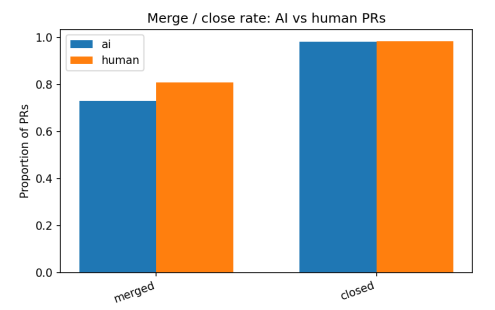
\includegraphics[height=2.2in]{figures/rq1_merge_close_rate_bar.png}\hfill
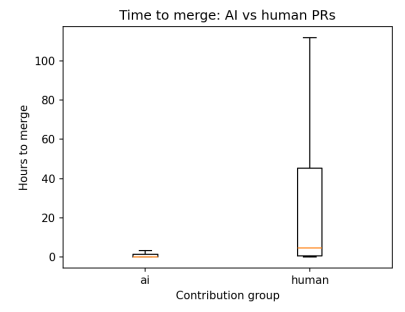
\includegraphics[height=2.2in]{figures/rq1_time_to_merge_boxplot.png}
\caption{RQ1. Left: merge and close rate of AI vs.\ human PRs. Right: time to merge of merged PRs in hours (outliers hidden).}
\label{fig:rq1}
\end{figure*}

\textbf{RQ1 -- Observations.} AI PRs are merged less often than human PRs (72.9\% vs.\ 80.8\%, $-7.9$ points, OR 0.64), a small effect ($\varphi\approx0.08$). Closing rates are nearly identical (98.1\% vs.\ 98.4\%, $p=0.107$), so almost every PR is resolved and the gap lies between merged and closed-without-merge (25.2\% of AI PRs vs.\ 17.6\% of human PRs). Among merged PRs, AI PRs are merged much faster: median 0.046\,h ($\approx$2.7 minutes) vs.\ 4.55\,h; an AI PR takes longer than a human one in only 23\% of random pairs. AI PRs also receive fewer reviews (median 0 vs.\ 1).

\textbf{RQ2 -- Observations.} Human interaction with AI PRs is thinner on every volume metric: the median AI PR has 0 comments, 0 reviewers and 0 participants versus 1 for human PRs (Fig.~\ref{fig:rq2}, left). The largest effect is review approval: 13.5\% of AI PRs have an approving review vs.\ 47.5\% of human PRs (OR 0.17, $\varphi\approx0.36$). Clarification and approval language are about 4 times less likely in AI PRs (1.7\% vs.\ 7.1\%; 3.9\% vs.\ 14.5\%). Rejection language and requested changes are also rarer but less strongly (2.4\% vs.\ 4.1\%; 2.8\% vs.\ 4.1\%). Comment length and alternations have median 0 in both groups, so their significant tests reflect the share of PRs with any discussion rather than longer or more reciprocal exchanges. The first-response test shows no difference ($p=0.973$), but this metric is unreliable (see Threats).

\begin{figure*}[t]
\centering
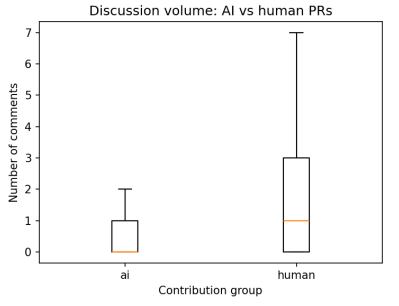
\includegraphics[height=2.2in]{figures/rq2_n_comments_boxplot.png}\hfill
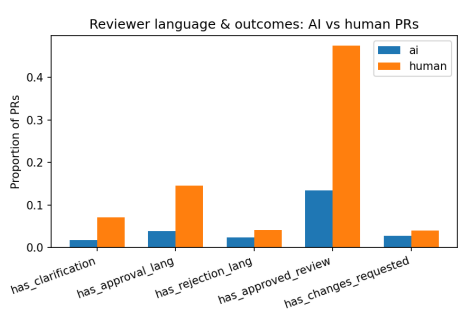
\includegraphics[height=2.2in]{figures/rq2_response_time_boxplot.png}
\caption{RQ2. Left: discussion volume (comments and reviews per PR, outliers hidden). Right: first response time of PRs in hours (outliers hidden).}
\label{fig:rq2}
\end{figure*}

\section{Discussion}
\textbf{Interpretation.} Taken together, AI PRs look less like contributions that are discussed and more like delegated output that is either accepted quickly or dropped. The combination of lower merge rate, near-zero review activity and merge times of a few minutes is consistent with the person who launched the agent merging its PR without a separate reviewer; the higher closed-unmerged share suggests that PRs which do not fit are simply closed. We did not mine who performed the merge, so this remains a hypothesis to test.

\textbf{Human--AI collaboration.} Collaboration around AI PRs is mostly implicit: few clarification requests and little approval language mean there is little visible negotiation between humans and agents. Review is the practice most reduced (OR 0.17 for approving reviews), which matters for quality assurance: if AI-authored changes receive less independent review than human ones, review effort and defect risk are decoupled from where the change came from. Note that our design sees only the \emph{human} side of the interaction, because agent replies are filtered out as bot noise.

\textbf{Implications.} Teams adopting agents may want explicit review policies for AI PRs, and tool builders could surface agents' rationale to invite the clarification questions that are currently rare.

\section{Threats to Validity}
\textbf{Timestamps and bots (internal).} Our GraphQL query requested \texttt{submittedAt} for reviews but the metric code reads \texttt{createdAt}; reviews are therefore ignored by first-response time and ordered incorrectly in the alternation count, and the AI PR author's own replies are typically removed as bot activity, so alternations are biased downward for AI PRs by construction. We mark both metrics ($^\dagger$) and draw no conclusion from them. \\
\textbf{Incomplete metadata.} Comment and review lists are capped (100/50/50), 3.0\% of sampled PRs could not be retrieved, and merger identity, labels, PR size and file changes were not mined. \\
\textbf{AI identification.} We trust AIDev's labels; human PRs may include unlabeled AI assistance, and the five agents are pooled. \\
\textbf{Classification errors.} Keyword lexicons miss negation, sarcasm and non-English text, and were not validated against manual labels. \\
\textbf{Dataset and repository specificity.} We analyse a 50\% sample of AI PRs; many PRs come from the same repositories, violating test independence and making $p$-values optimistic; results may not generalise beyond AIDev's repositories or period. \\
\textbf{Missing private context.} Discussions in chat, issue trackers, IDEs or pair sessions are invisible. \\
\textbf{Statistical.} Large $N$ makes tiny differences significant, hence our focus on effect sizes. \\

\section{Conclusion and Future Work}
On 21{,}740 mined PRs, AI-agent PRs are merged less often than human PRs but much faster, and attract far less human review and discussion; the sharpest gap is in approving reviews (13.5\% vs.\ 47.5\%). Future work would include fixing the timestamp handling and rerunning the analysis, mining merger identity and PR size, analyzing each agent separately, adding task-type classification, modeling merge outcome with logistic regression and repository-level random effects, and validating the language lexicons against manual labels.

\section*{AI-Use Disclosure}
An AI assistant (Claude) was used to format this LaTeX report from the authors' own pipeline outputs and to compute effect sizes from the printed test statistics. Data collection, cleaning and statistical analysis were run by the authors in the replication notebook; the authors reviewed and verified all results and interpretations.

\begin{thebibliography}{99}
\bibitem{li2025rise} H.~Li, H.~Zhang, and A.~E.~Hassan, ``The rise of AI teammates in software engineering (SE) 3.0: How autonomous coding agents are reshaping software engineering,'' arXiv:2507.15003, 2025. Dataset: \url{https://huggingface.co/datasets/hao-li/AIDev}.
\bibitem{githubgql} GitHub, ``GitHub GraphQL API documentation,'' \url{https://docs.github.com/en/graphql}.
\bibitem{mannwhitney} H.~B.~Mann and D.~R.~Whitney, ``On a test of whether one of two random variables is stochastically larger than the other,'' \emph{Ann.\ Math.\ Statist.}, vol.~18, no.~1, pp.~50--60, 1947.
\bibitem{scipy} P.~Virtanen \emph{et al.}, ``SciPy 1.0: Fundamental algorithms for scientific computing in Python,'' \emph{Nature Methods}, vol.~17, pp.~261--272, 2020.
\bibitem{gousios2014pull}
G. Gousios and A. Zaidman, ``A dataset for pull-based development research,'' in \emph{Proc. 11th Working Conf. Mining Software Repositories (MSR)}, 2014, pp. 368--371, doi: 10.1145/2597073.2597122.
\bibitem{kalliamvakou2016github}
E. Kalliamvakou, G. Gousios, K. Blincoe, L. Singer, D. M. German, and D. Damian, ``An in-depth study of the promises and perils of mining GitHub,'' \emph{Empirical Software Engineering}, vol. 21, no. 5, pp. 2035--2071, 2016, doi: 10.1007/s10664-015-9393-5.
\bibitem{rigby2015review}
P. C. Rigby, A. Bacchelli, G. Gousios, and M. Mukadam, ``A mixed methods approach to mining code review data: Examples and a study of multi-commit reviews and pull requests,'' in \emph{The Art and Science of Analyzing Software Data}. Morgan Kaufmann, 2015, pp. 231--255.
\bibitem{copilot2022pair}
S. Imai, ``Is GitHub Copilot a substitute for human pair-programming? An empirical study,'' in \emph{Proc. IEEE/ACM 44th Int. Conf. Software Engineering: Companion Proc. (ICSE-Companion)}, 2022, pp. 319--321, doi: 10.1109/ICSE-Companion55297.2022.9793778.
\bibitem{li2026aidev}
H. Li, H. Zhang, and A. E. Hassan, ``AIDev: Studying AI coding agents on GitHub,'' arXiv:2602.09185, 2026. [Online]. Available: \url{https://arxiv.org/abs/2602.09185}
\bibitem{goldkrinke2022ethics}
N. E. Gold and J. Krinke, ``Ethics in the mining of software repositories,'' \emph{Empirical Software Engineering}, vol. 27, art. no. 17, 2022, doi: 10.1007/s10664-021-10057-7.
\bibitem{mazloomzadeh2026}
I. Mazloomzadeh, M. M. Morovati, and F. Khomh, ``How do AI coding agents contribute to software development? An empirical study of agentic pull requests,'' arXiv:2607.21832, 2026. [Online]. Available: \url{https://arxiv.org/abs/2607.21832}
\end{thebibliography}

\end{document}